\section{Ethylene oxidation in a partially-stirred reactor}

\citet{manzello2007soot} utilized NIST well-stirred reactor (WSR) connected to a flow reactor to study soot formation during ethylene oxidation at equivalence ratios of 1.9, 2.0, and 2.1, and provided PSD measurements at the end of flow reactor using nano-differential mobility analyzer (Nano-DMA). The WSR has the same size of the reactor used by \citet{manzello2007soot} and explained in Sec.\ref{sec:psrvalid}. The flow reactor is 70 cm long with an inner diameter of 5.1 cm. A coupled PSR-PFR reactor model of omnisoot was used with the same dimensions to study gas chemistry and soot inception during the combustion and flow evolution in the device. The nominal residence time, $\tau$ of flow in the PSR is 11 ms~\citet{manzello2007soot}. The reactants are assumed to enter PSR at 300 K with an inlet mass flow rate, $\dot{m}_{in}=\rho V / \tau$ where $\rho$ was calculated at reactor temperature of 1723 K suggested by~\citet{lenhert2009effects}. The PFR is assumed to be adiabatic. The calculated average axial velocity in the PFR is 14.5 m/s close to the values suggested by~\citet{manzello2007soot}. KAUST mechanism was used The inception and PAH adsorption scaling factors were varied to match the PSD predicted by each inception model with the measurements at different $\phi$s.

\begin{figure}[H]
	\centering
	\begin{tikzpicture}
		\draw (0, 0) node[inner sep=0] 	{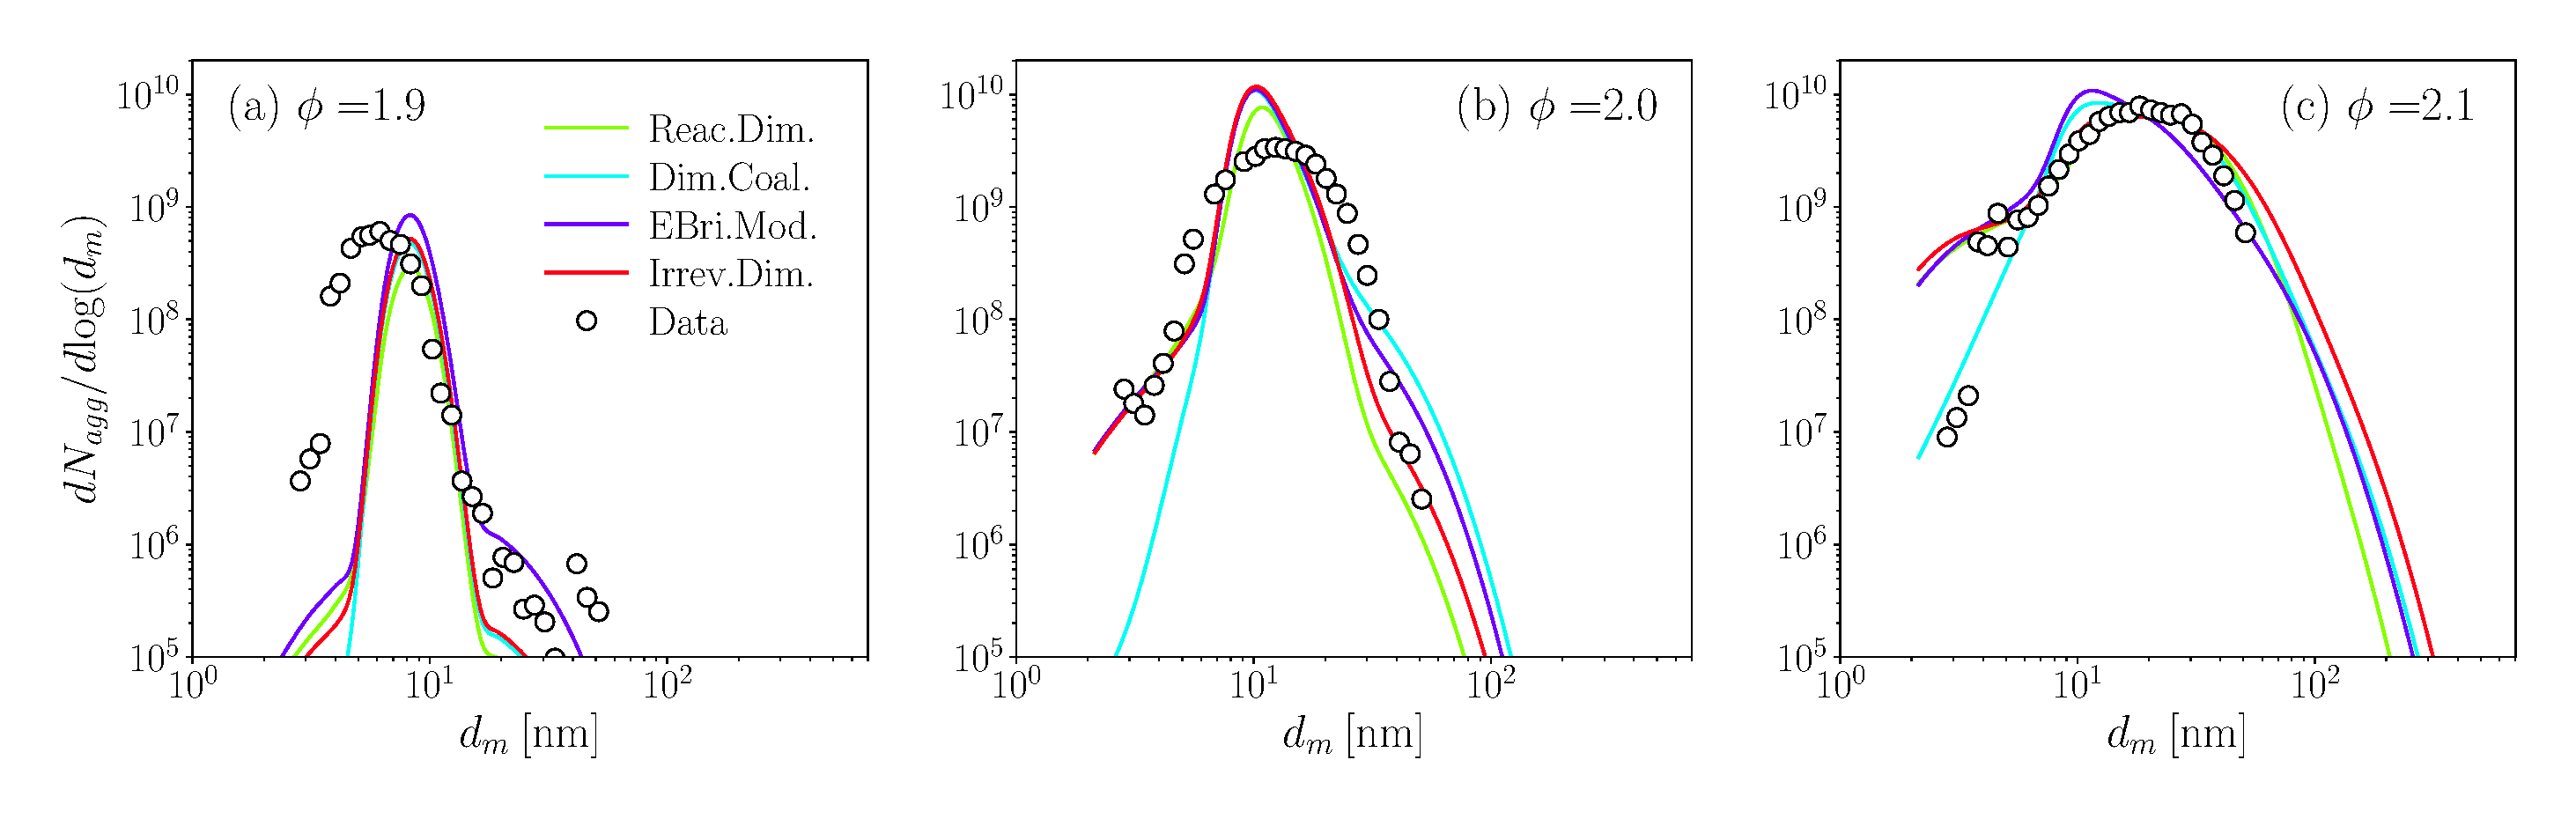
\includegraphics[width=1\textwidth]{Figures/Results/PSR/PSD_eq_ratio_log.pdf}};
		\draw (-3.1, 0.6) node {\tiny{\cite{manzello2007soot}}};
		\draw (1.95, 0.66) node {\tiny{\cite{manzello2007soot}}};
		\draw (5.5, -1.28) node {\tiny{\cite{manzello2007soot}}};
	\end{tikzpicture}
	\caption{The particle size distribution at the end of PFR for $\phi$=1.9 (a), 2.0 (b), and 2.1 (c) obtained using KAUST mechanism and different inception models calibrated to match the predictions with measurement~\citep{manzello2007soot}.}
	\label{fig:psrpfr_psd} 
\end{figure}


\begin{figure}[H]
	\centering
	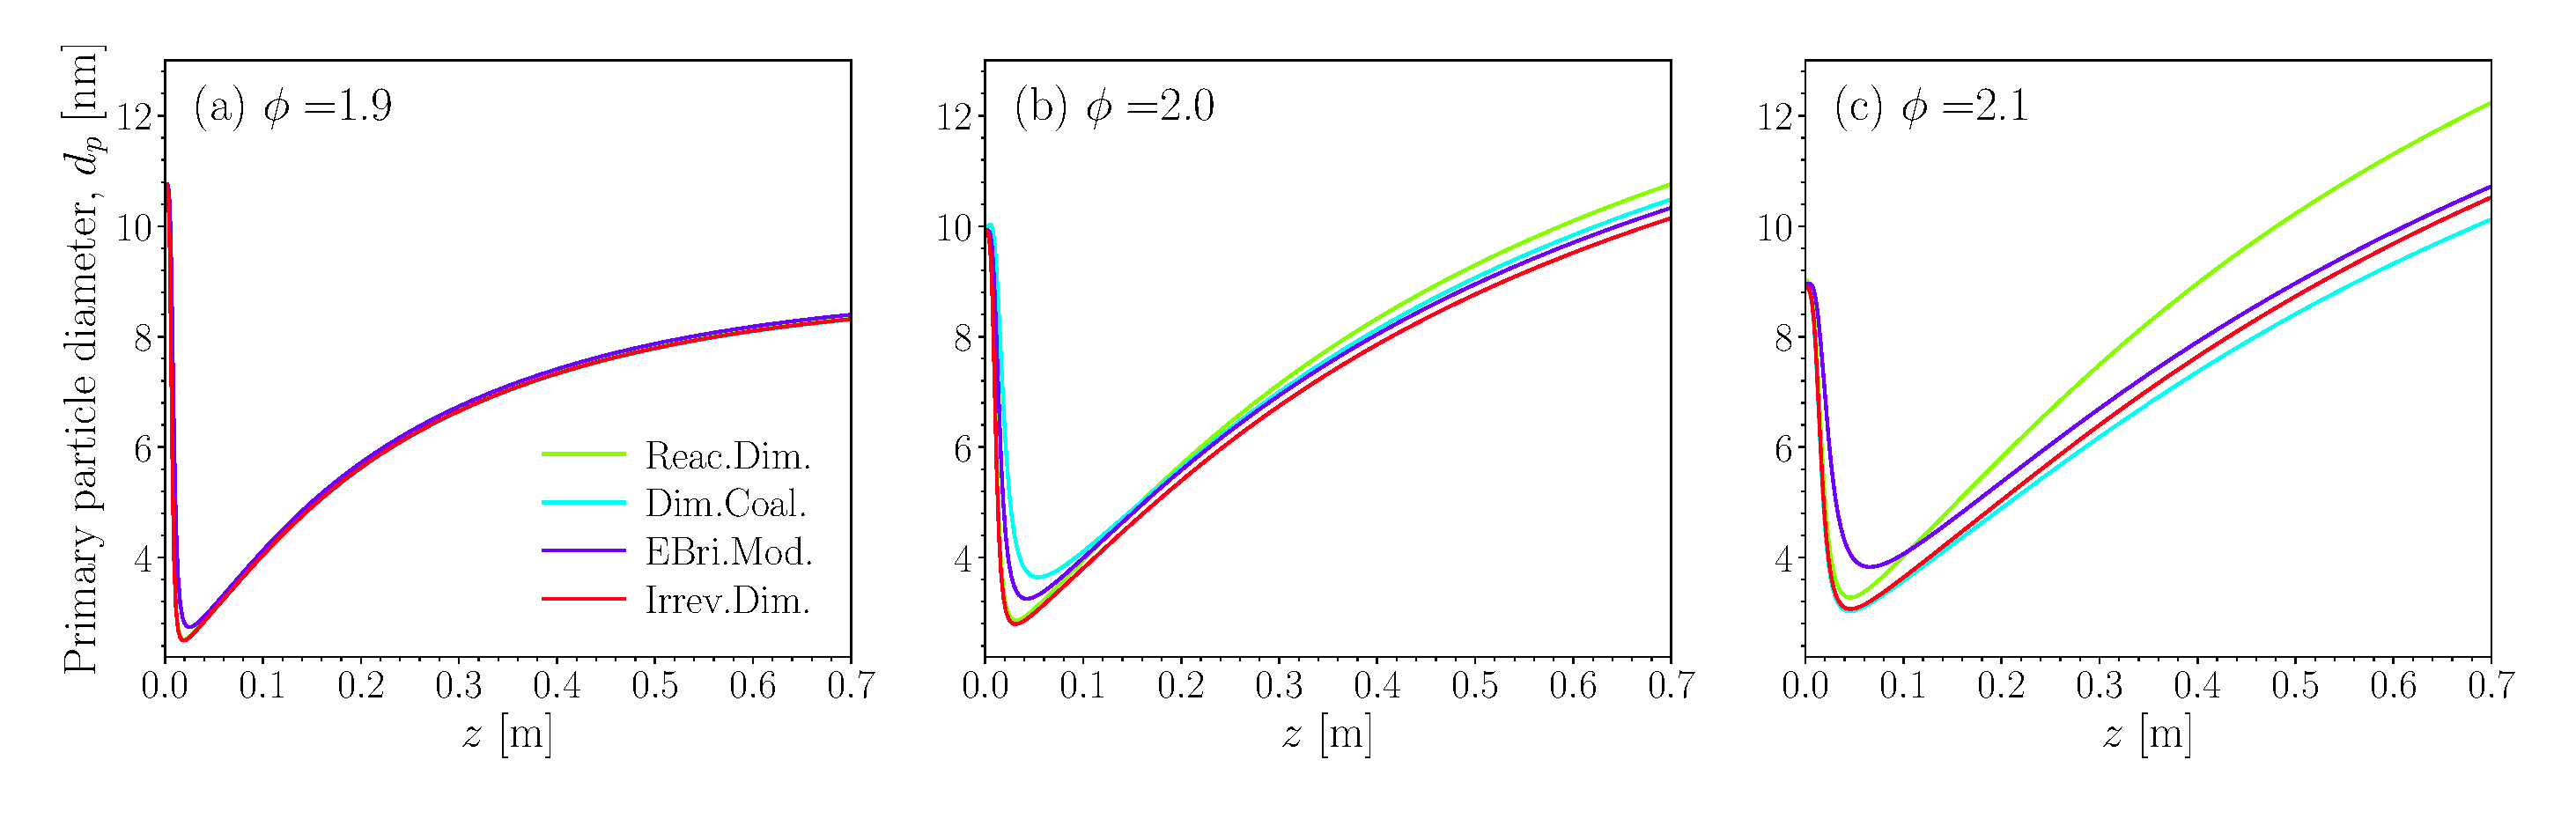
\includegraphics[width=1\textwidth]{Figures/Results/PSR/d_p_eq_ratio_all_single_mech.pdf}
	\caption{The primary particle diameter, $d_p$ along the PFR for $\phi$=1.9 (a), 2.0 (b), and 2.1 (c) obtained using KAUST mechanism and different inception models calibrated to match the predictions with measurement~\citep{manzello2007soot}.}
	\label{fig:psrpfr_dp} 
\end{figure}

\begin{figure}[H]
	\centering
	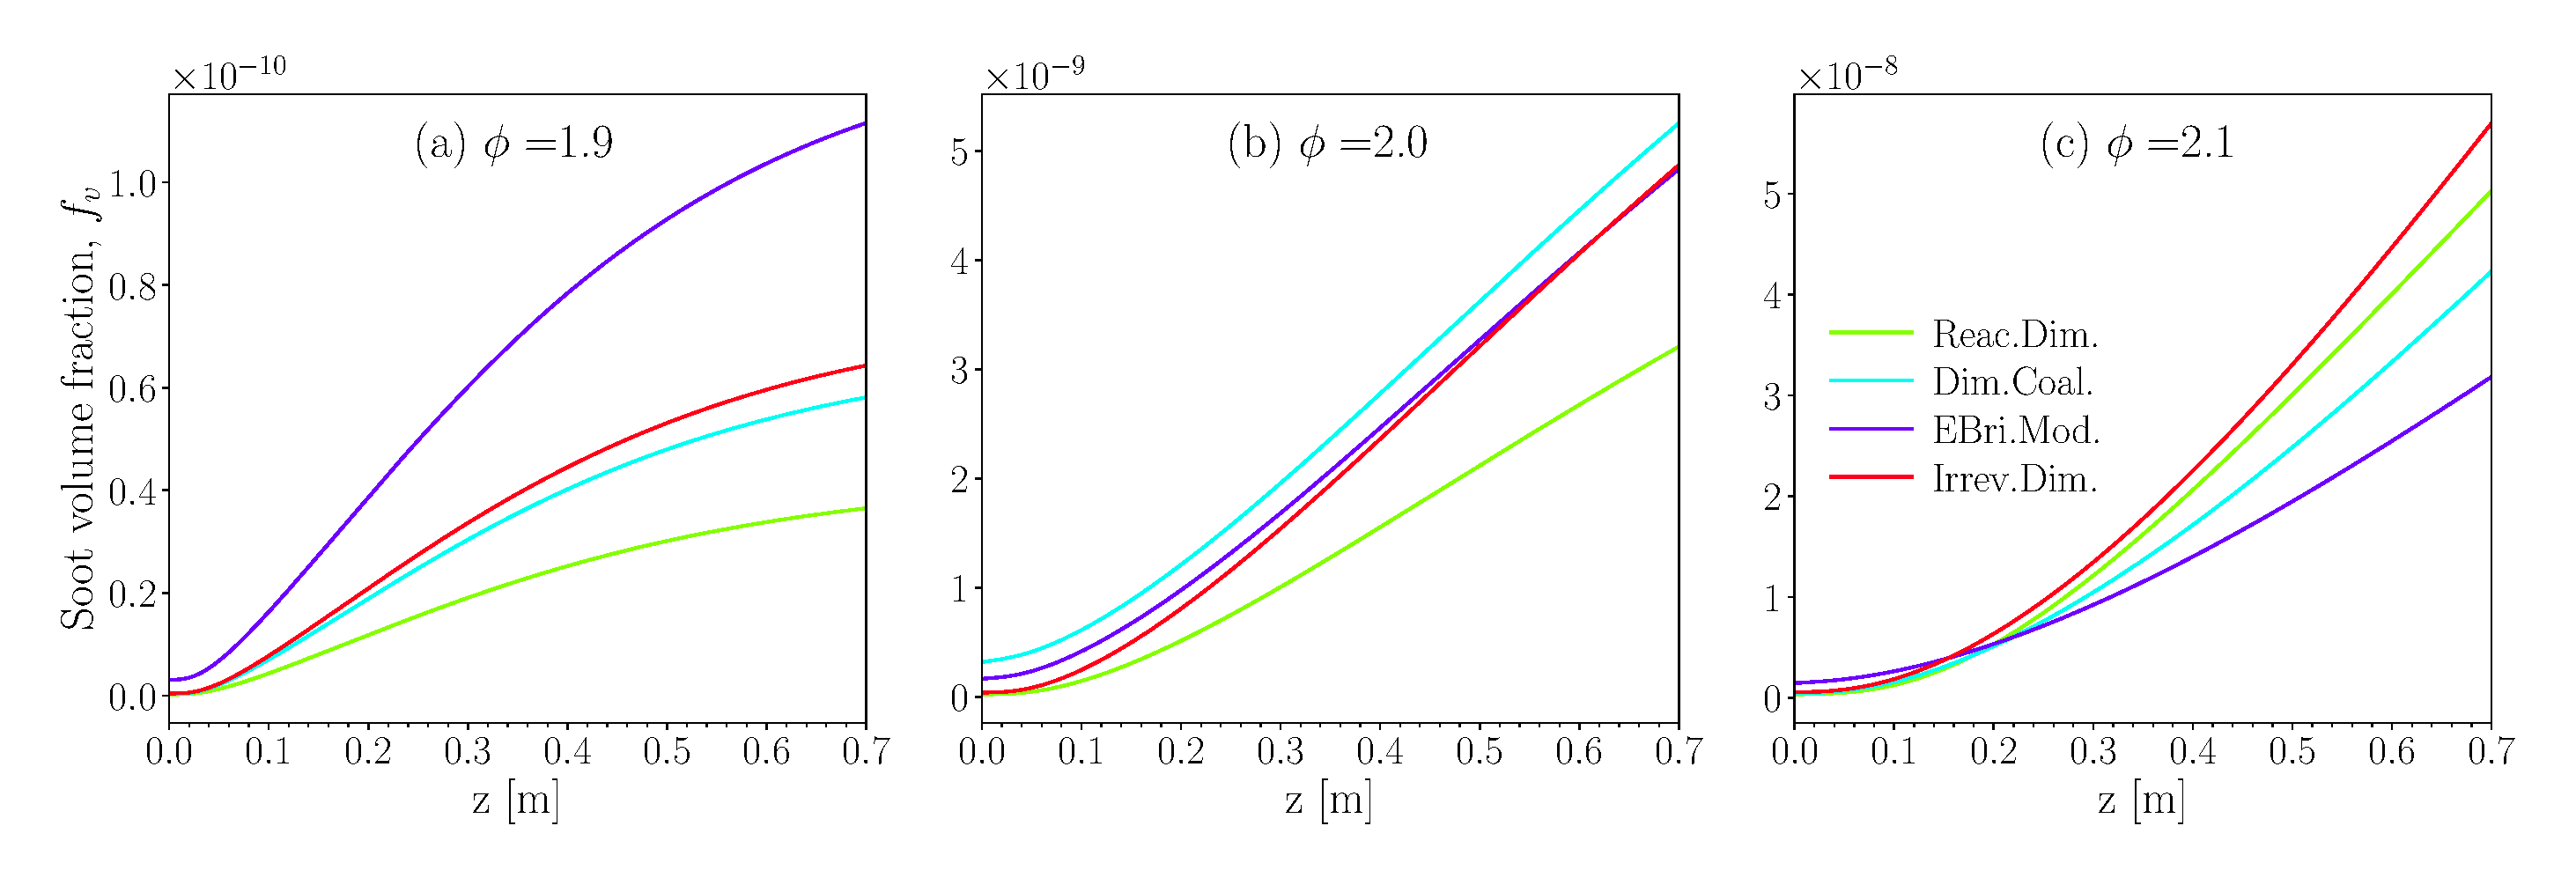
\includegraphics[width=1\textwidth]{Figures/Results/PSR/f_v_eq_ratio_all_single_mech.pdf}
	\caption{The soot volume fraction, $f_v$ along the PFR for $\phi$=1.9 (a), 2.0 (b), and 2.1 (c) obtained using KAUST mechanism and different inception models calibrated to match the predictions with measurement~\citep{manzello2007soot}.}
	\label{fig:psrpfr_fv} 
\end{figure}

\begin{figure}[H]
	\centering
	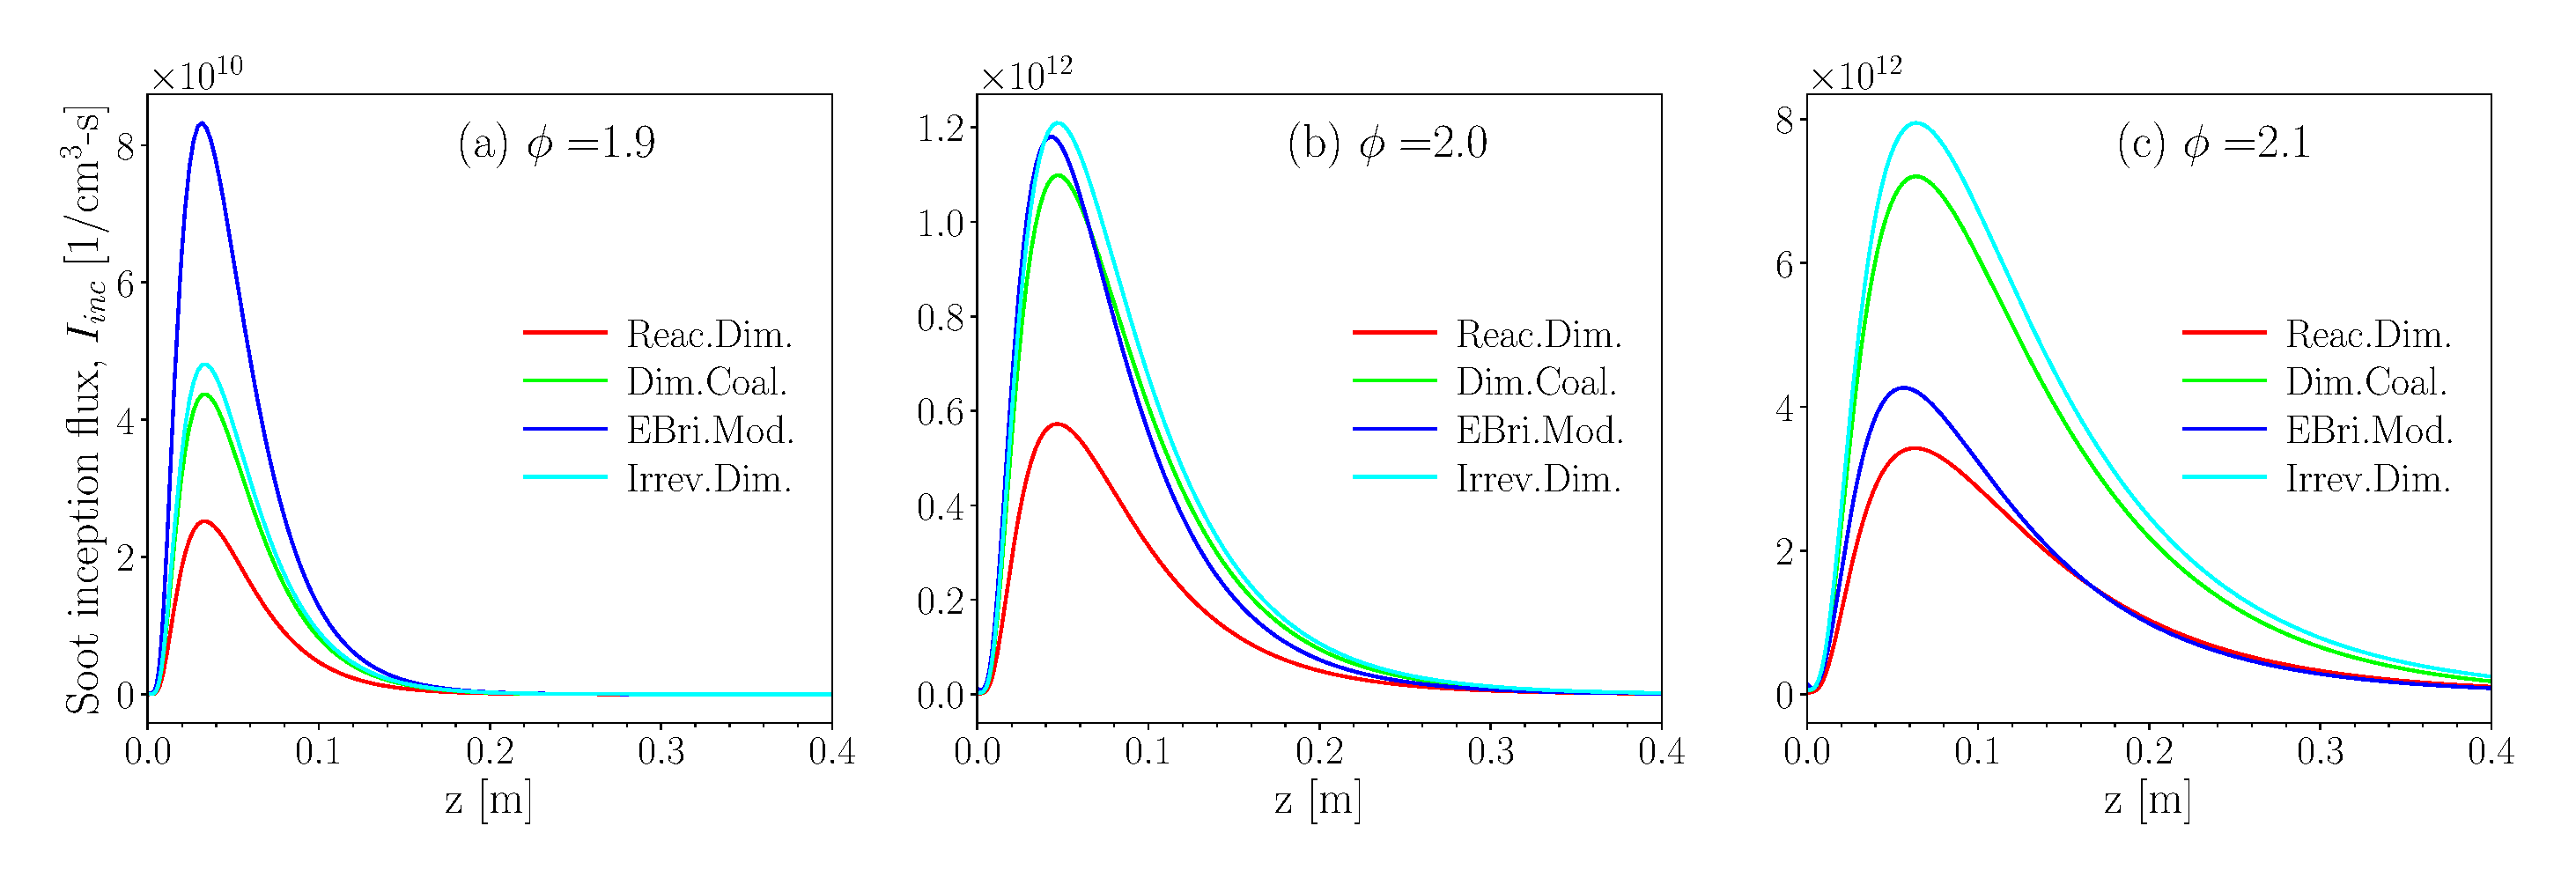
\includegraphics[width=1\textwidth]{Figures/Results/PSR/I_inc_eq_ratio_all_single_mech.pdf}
	\caption{The soot inception flux, $I_{inc}$ along the PFR for $\phi$=1.9 (a), 2.0 (b), and 2.1 (c) obtained using KAUST mechanism and different inception models calibrated to match the predictions with measurement~\citep{manzello2007soot}.}
	\label{fig:psrpfr_Iinc} 
\end{figure}

\begin{figure}[H]
	\centering
	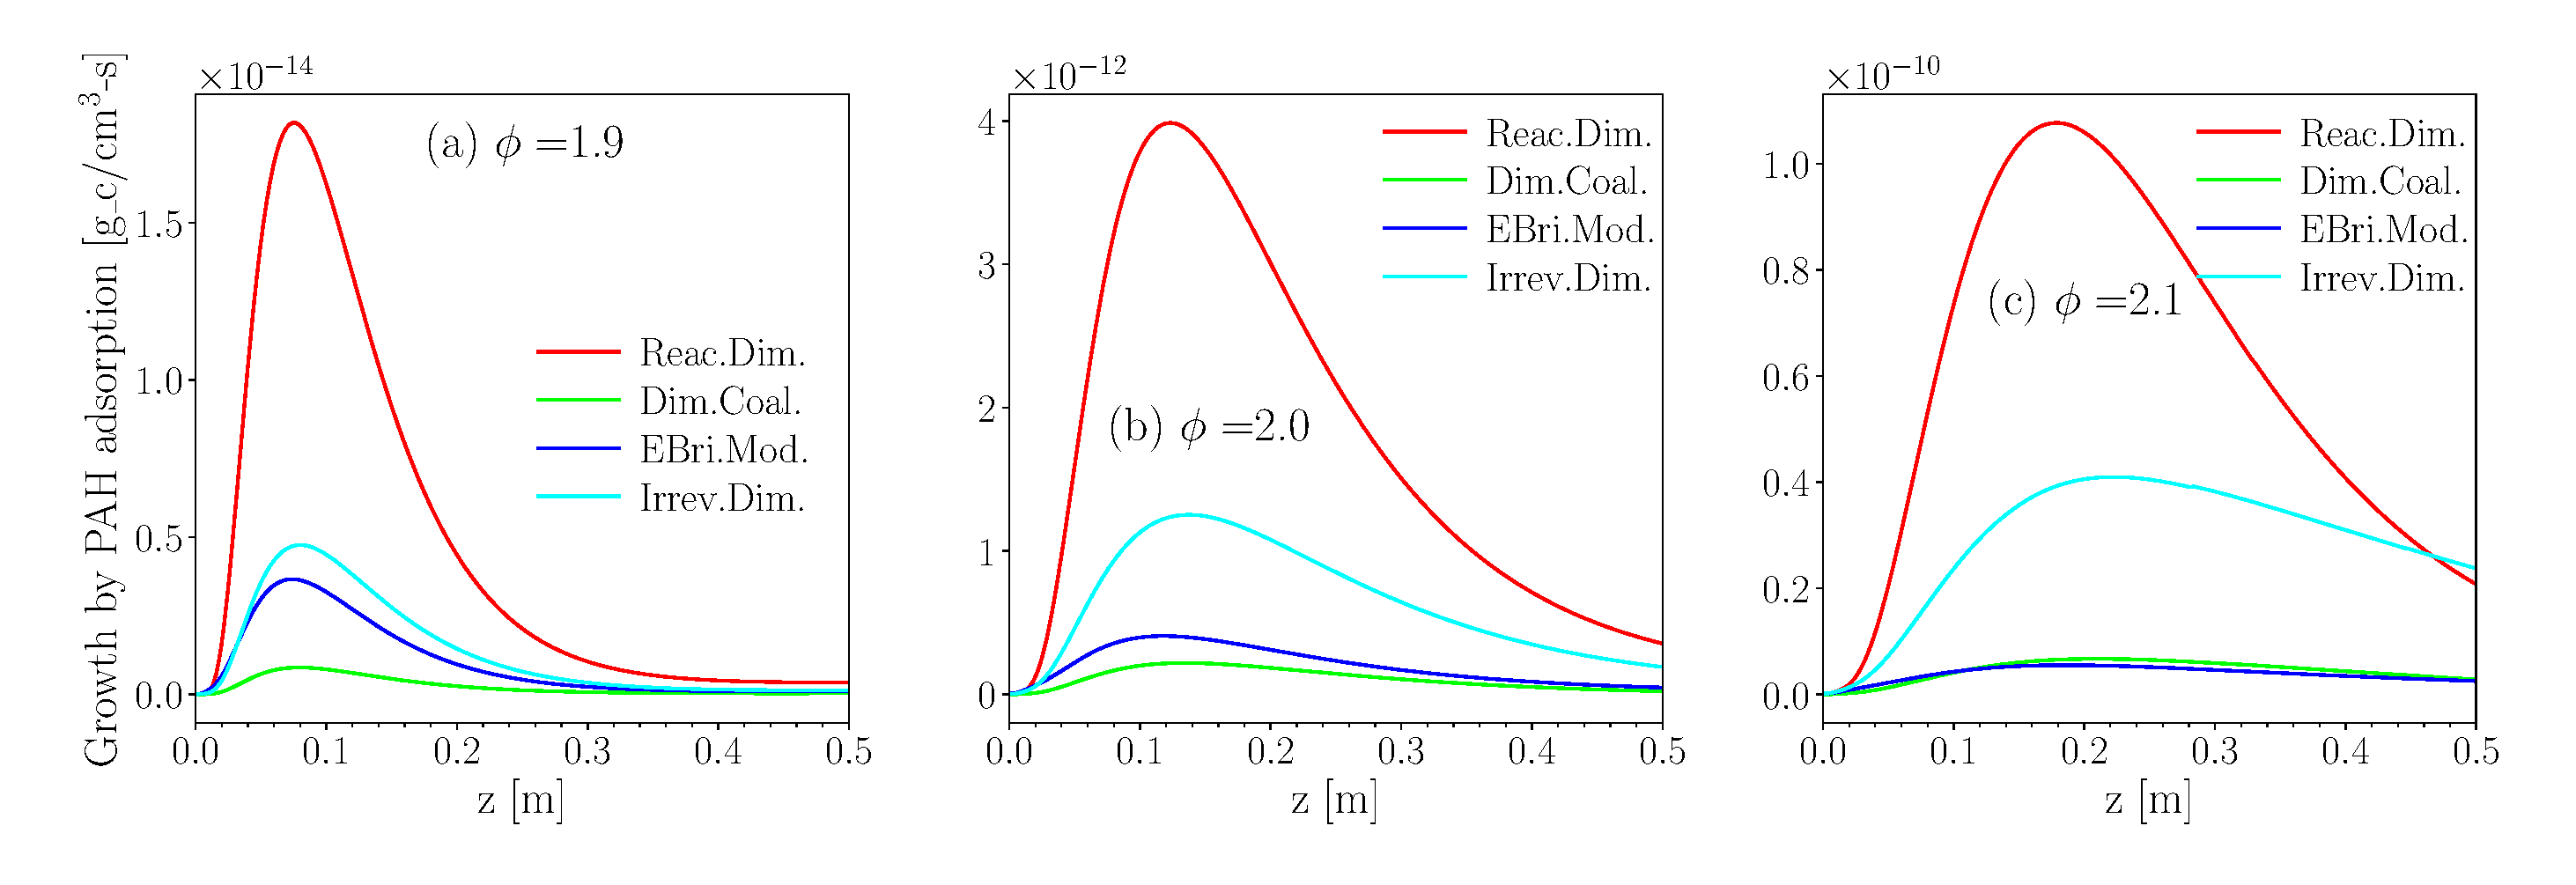
\includegraphics[width=1\textwidth]{Figures/Results/PSR/PAH_rate_eq_ratio_all_single_mech.pdf}
	\caption{The carbon growth rate by PAH adsorption rate along the PFR for $\phi$=1.9 (a), 2.0 (b), and 2.1 (c) obtained using KAUST mechanism and different inception models calibrated to match the predictions with measurement~\citep{manzello2007soot}.}
	\label{fig:psrpfr_PAHads} 
\end{figure}

\begin{figure}[H]
	\centering
	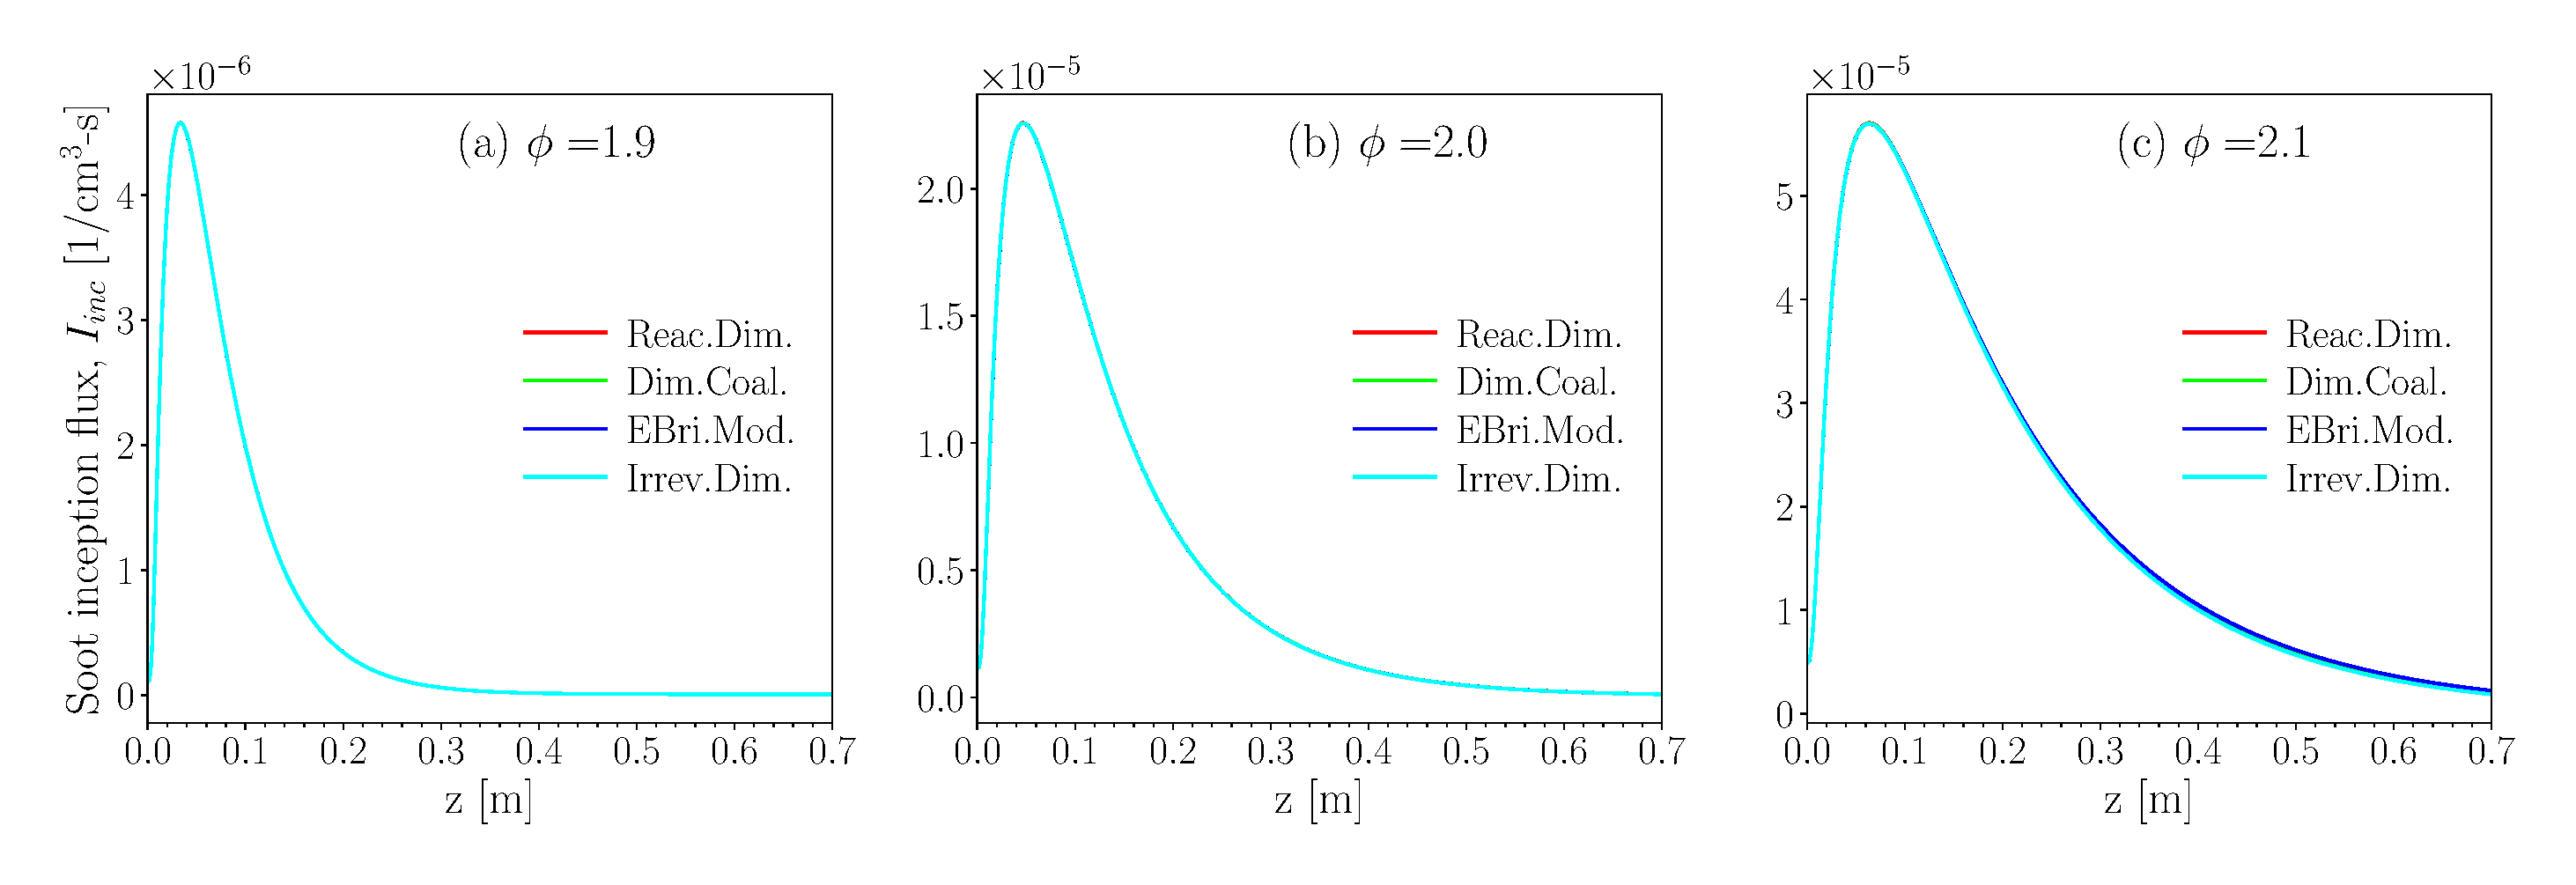
\includegraphics[width=1\textwidth]{Figures/Results/PSR/A2R5_eq_ratio_all_single_mech.pdf}
	\caption{The mole fraction of acenaphthylene, A2R5 along the PFR for $\phi$=1.9 (a), 2.0 (b), and 2.1 (c) obtained using KAUST mechanism and different inception models calibrated to match the predictions with measurement~\citep{manzello2007soot}.}
	\label{fig:psrpfr_A2R5} 
\end{figure}